\documentclass{article}
\usepackage[utf8]{inputenc}
\usepackage{caption}
\usepackage{amsmath}
\usepackage{amssymb}
\usepackage{mathtools}
\usepackage{multicol}
\usepackage{graphicx}
\usepackage{wrapfig}
\usepackage{float}
\usepackage[makeroom]{cancel}
\usepackage{mhchem}
\usepackage{pst-plot}

\graphicspath{ {../images/} }

\renewcommand{\familydefault}{\sfdefault}
\renewcommand{\baselinestretch}{1.5} % line spacing
\newcommand{\fline}{\par\noindent\rule{\textwidth}{0.1pt}} % horizontal line (wide)

\title{Topic 5 Oxidation \& Reduction\\Lesson 3 - Electorlytic Cells}
\author{Peter Zhang}

\begin{document}

\maketitle
\tableofcontents
\newpage

% lesson 
\section{Electrolytic Cell}
\begin{enumerate}
\item Non-spontaneous reactions\\- Driven by electrical energy
\item Reactants are present as an electrolyte\\- A liquid that is molten or aqueous ionic compound
\item Electric current passes through the electrolyte + a redox rxn occurs\\- removes charges on ions + forms electrically neutral products (once this finishes it is finished)
\item Water complicates the measurements made for a circuit $\rightarrow$ deeper understanding required when creating electrolyte solutions!
\begin{figure}[H]
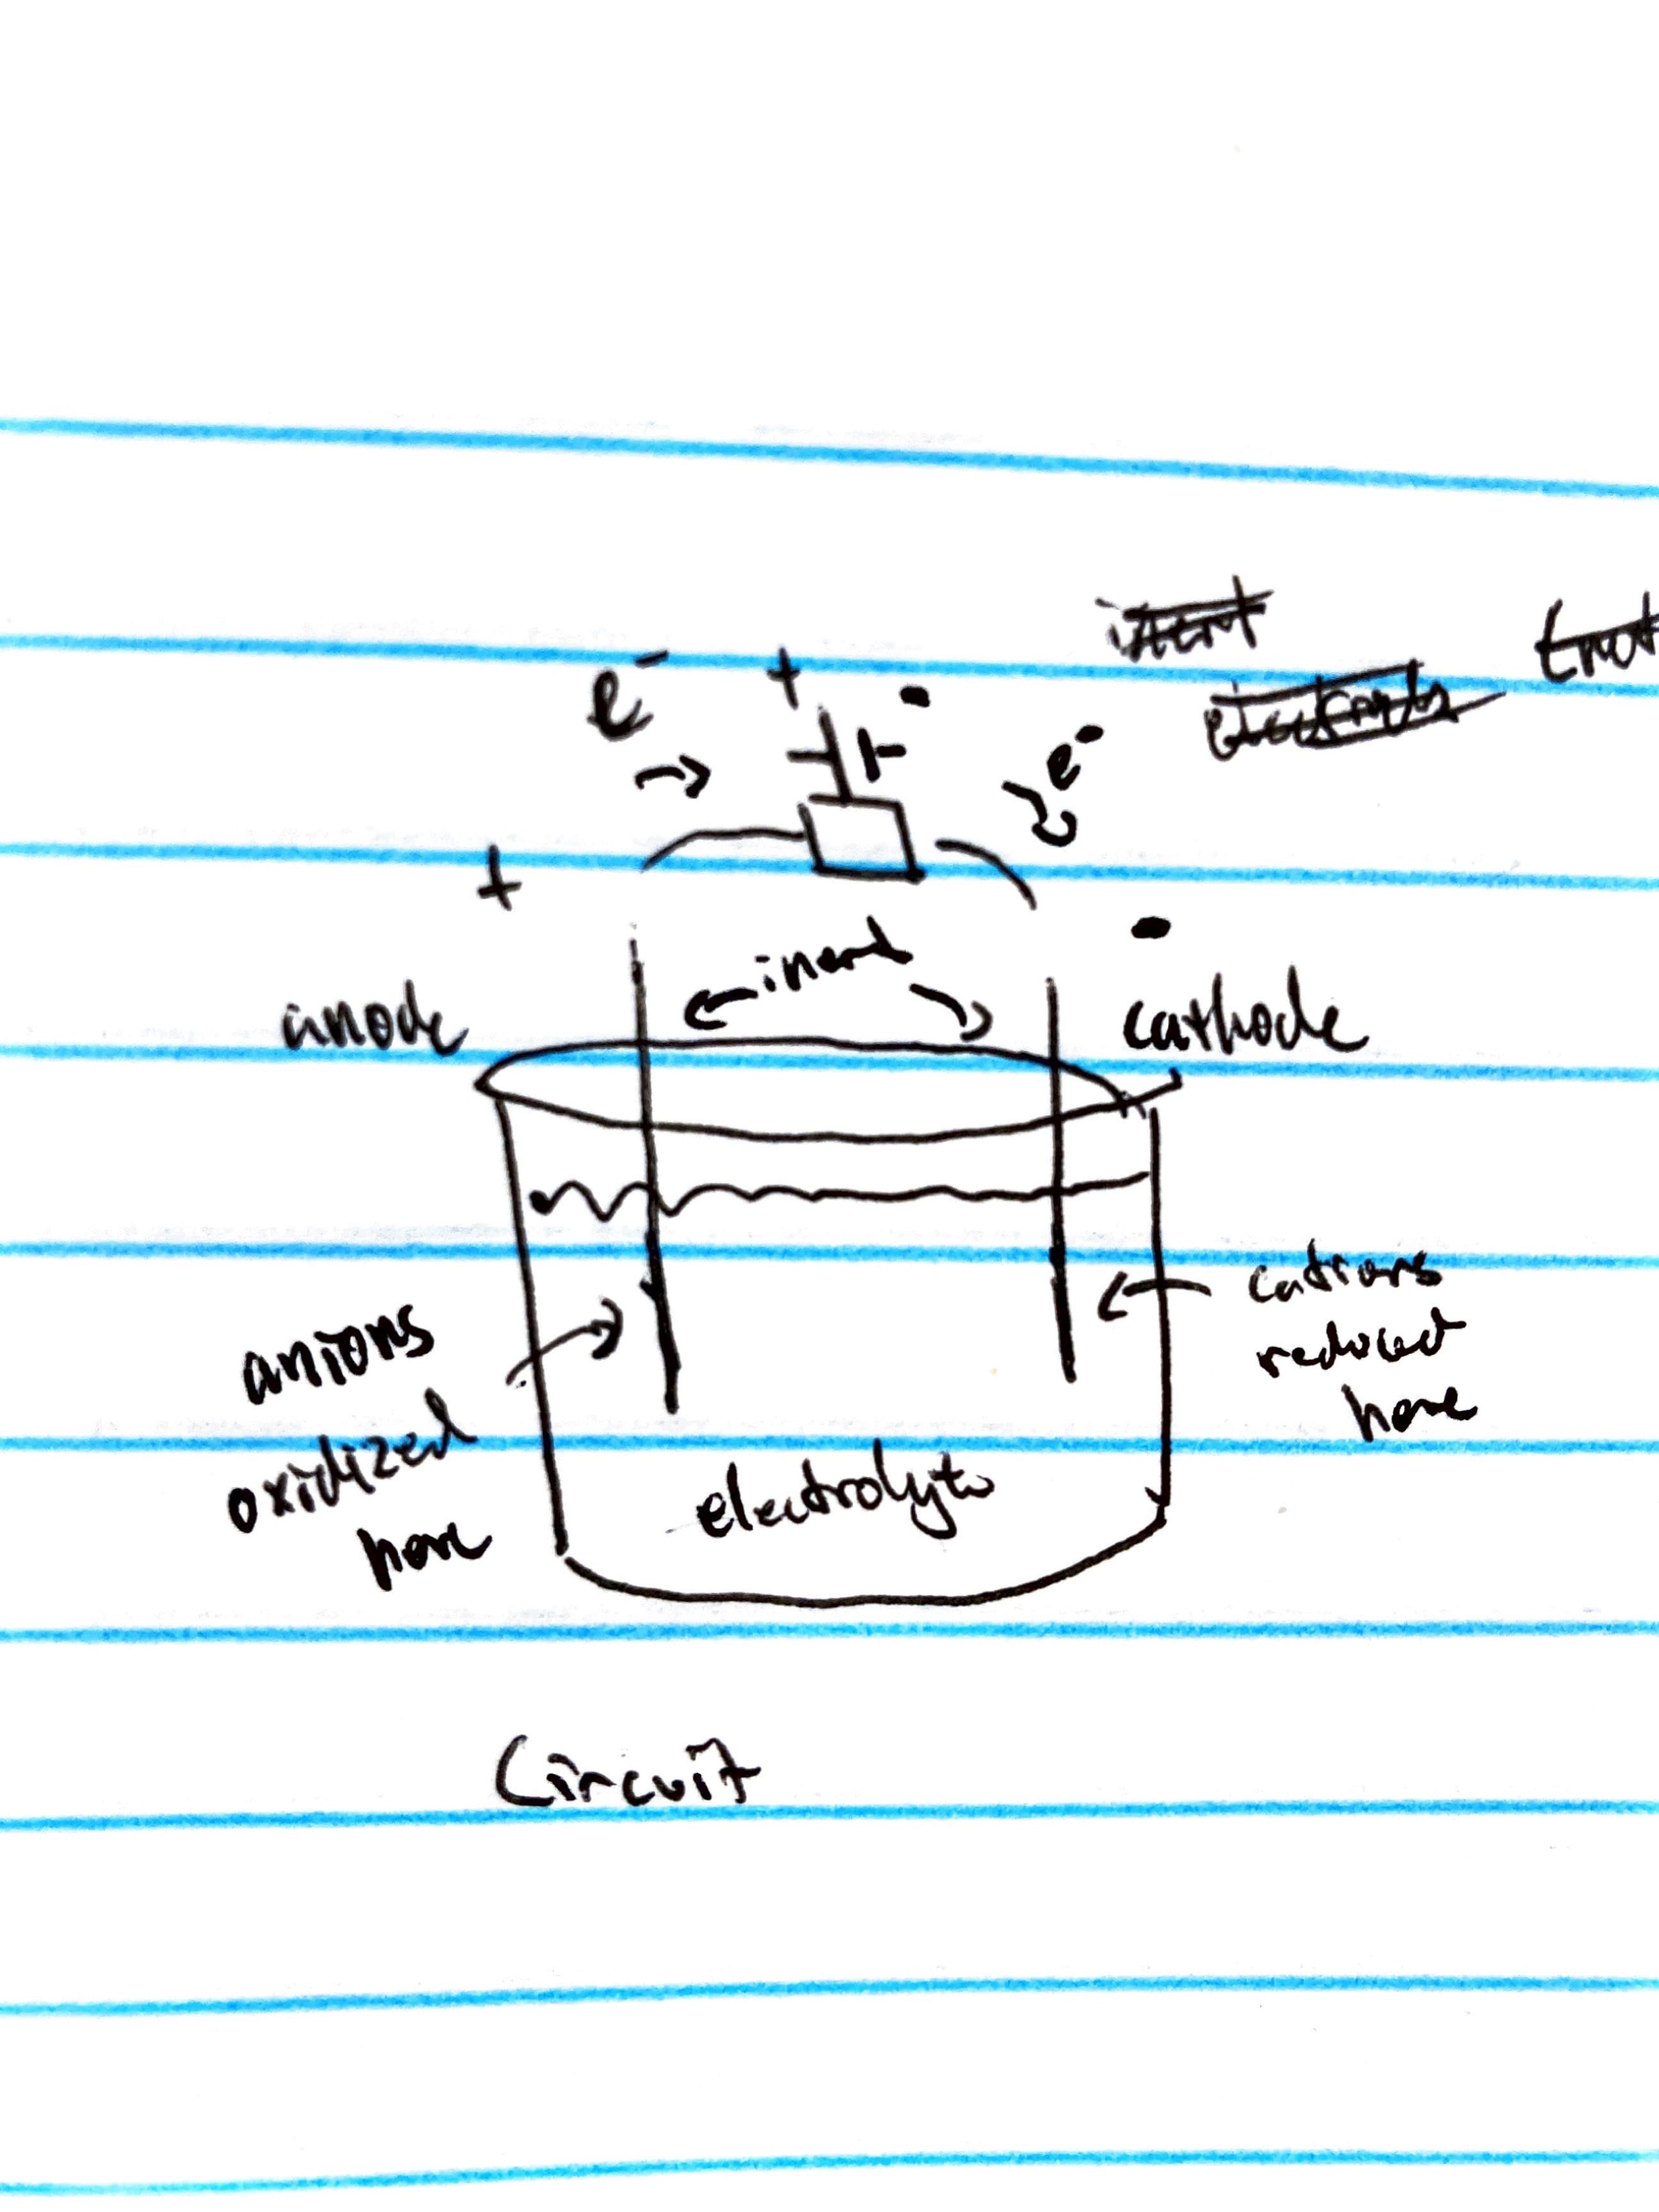
\includegraphics[width=0.6\textwidth]{5.3circuit1.JPG}
\captionof{figure}{Circuit diagram}
\end{figure}


\subsection{Types}
\begin{enumerate}
\item Molten Salts
\begin{enumerate}
\item Only the ions from the compounds are present:
Example: LiCl (oxidation [anode])\ \ \ \ (reduction [cathode])
$$\ce{2Cl- (g) \rightarrow Cl2 (g) + 2e-}\ \ \ \ce{2Li+ (aq) + 2e- \rightarrow 2Li(g)}$$
\item \textbf{MULTIPLE REDOX reactions can occur!}
\end{enumerate}
\end{enumerate}

\item Aqueous Solutions
\begin{enumerate}
\item Can be influenced by the presence of \ce{H2O}
\item \ce{H2O} can be oxidized or reduced!
\item because \textbf{\ce{H2O}} can be oxidized or reduced
\begin{enumerate}
\item Relative $E^{o}$ of ions
\item Concentration of ions in electrolyte\\How much solute vs solvent
\item Nature of electrodes!\\inert = no say in equation\\specific types of electrodes may influence different ions from H2O
\end{enumerate}
\item \textbf{\ce{H2O} Based Circuit} (\ce{NaOH (aq) -> Na+ (aq) + OH- (aq)})
\begin{enumerate}
\item Cathode is positive, Anode is negative
\item At the cathode: $\ce{Na+ (aq) + e- -> Na(s)\ \ \ E^{o} = -2.71V}\\\ce{2H2O(l) + 2e- -> H2 (g) + 2OH-\ \ \ E^{o}=-0.83V}$
\item At the anode: $\ce{4OH- (aq) -> 2H2O(l) + O2(g) + 4e-\ \ \ E^{o}=-0.40V}\\\ce{2H2O(l) -> 4H+ (aq) + O2 (g) + 4e-\ \ \ E^{o}=-1.23V}$
\end{enumerate}
\item We have two possible reactions and so we must pick or decide which one will be favored
\item H2O\\if \textbf{LOW CONCENTRATION OF IONS}:\\\ce{2H2O(l) -> 2H2(g) + O2(g)} 
\item NaCl\\if \textbf{HIGH CONCENTRATION}:\\\ce{NaCl(aq) -> Na+ (aq) + Cl- (aq)}\\\ce{Na+ (aq) + e- -> NO(s)\ \ \ $E^{o} = -2.71V$}\\\ce{2H2O(l) + 2e- -> H2(g) + 2OH-\ \ \ $E^{o}=-0.83V$}\\At the anode:
\ce{2Cl- (aq) -> Cl2(g) + 2e-\ \ \ $-E^{o}=-1.36V$}\\\ce{2H2O(l) -> 4H+ + O2(g) + 4e-\ \ \ $-E^{o}=-1.23V$}

\item Overall...\\$$\ce{2NaCl(aq) + 2H2O(l) -> H2(g) + Cl2(g) + Na+ (aq) + 2OH- (aq)}$$
\end{enumerate}
\item If concentration of NaCl is low, H2O is oxidized
\item If concentration is greater than 25\%, then \ce{Cl-} is oxidized
\end{enumerate}

If we use a Cu electrode
\begin{figure}
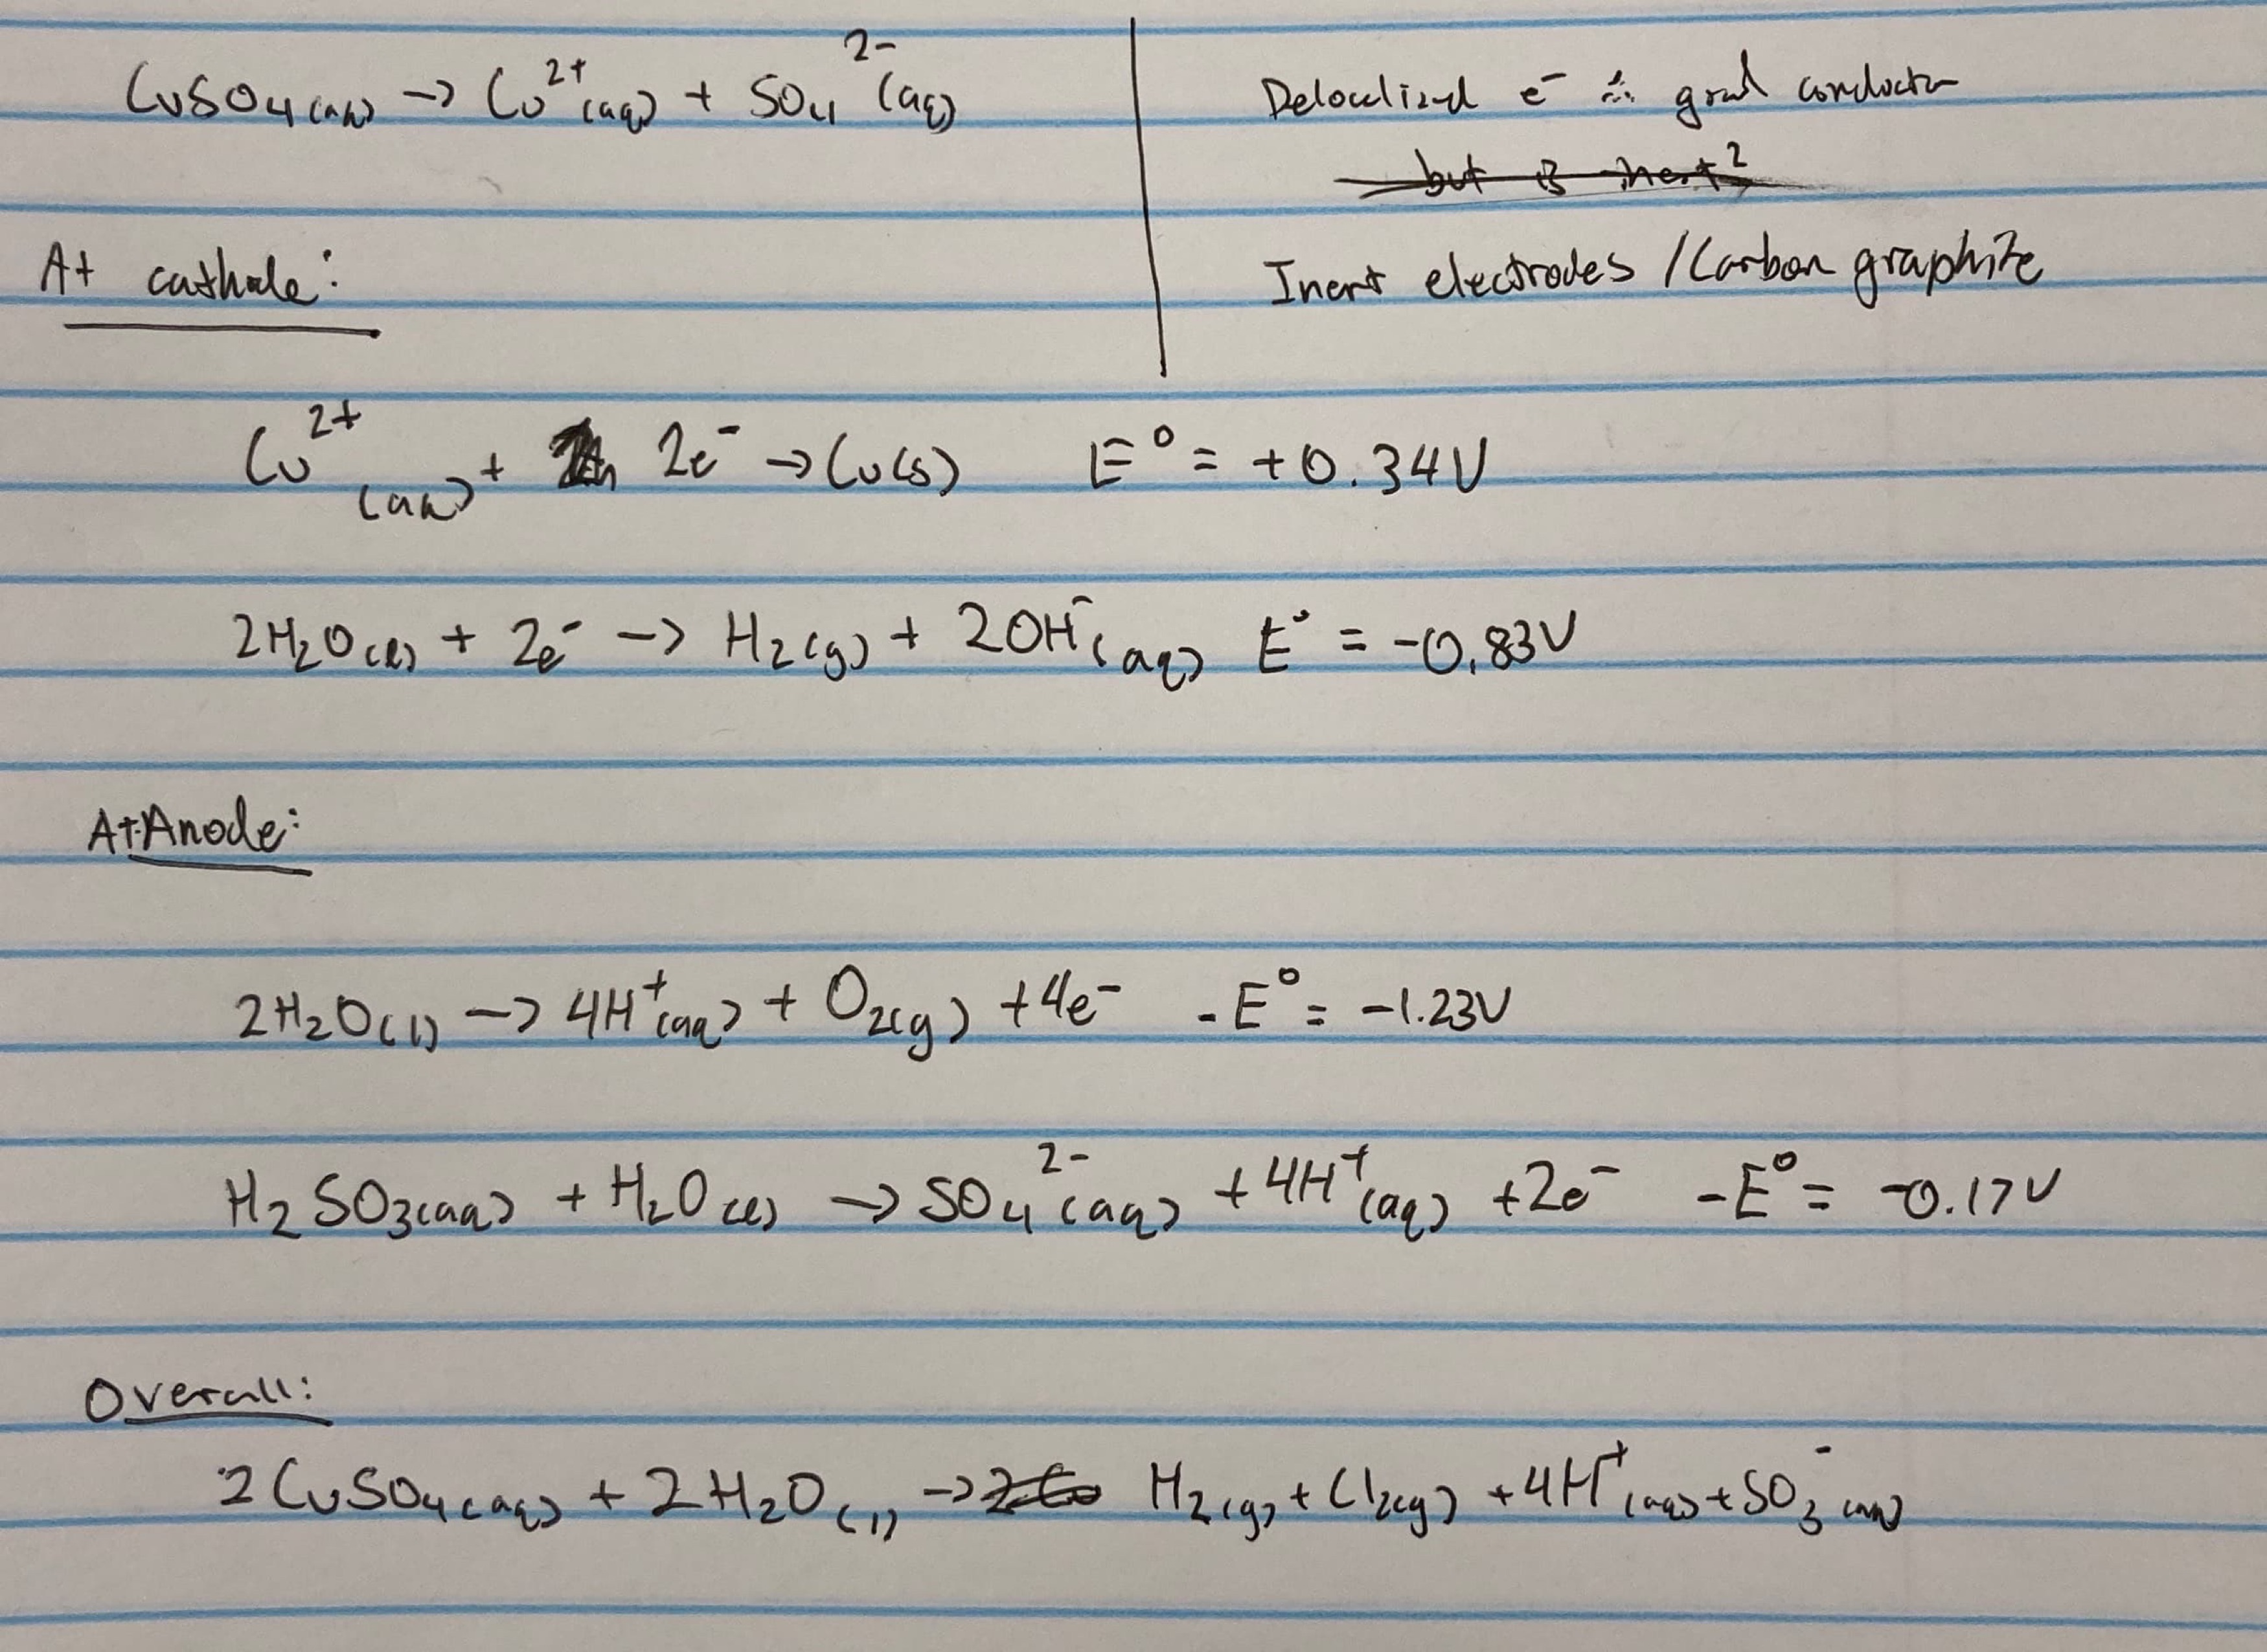
\includegraphics[width=\textwidth]{5.3circuit2.jpg}
\captionof{figure}{How to solve Question}
\end{figure}
The next reaction is movement of \ce{Cu2+} from where it is produced at the anode to the cathode where it is discharged.

This is an example of electroplating\\Can deposit a layer of metal on top of another metal


\end{document}